\documentclass{PoS}

% Shortcuts
\newcommand{\aap}{AAP}
\newcommand{\pasp}{PASP}
\newcommand{\url}[1]{\href{#1}{#1}}

\title{Gammapy -- A prototype for the CTA science tools}
\ShortTitle{Gammapy -- A prototype for the CTA science tools}

\author{
% TODO: put Matteo as Speaker?
\speaker{Christoph Deil}$^a$,
Julien Lefaucheur$^b$,
R\'egis Terrier$^c$,
Bruno Kh\'elifi$^c$,
Matthew Wood$^d$,
Roberta Zanin$^a$,
Lars Mohrmann$^e$,
Nachiketa Chakraborty$^a$,
Jason Watson$^a$,
Rub\'en L\'opez Coto$^a$,
Stefan Klepser$^f$,
Matteo Cerruti$^g$,
Jean-Philippe Lenain$^g$,
Fabio Acero$^h$,
Arache Djannati-Ata{\"\i}$^c$,
Santiago Pita$^c$,
Zeljka Bosnjak$^i$,
Jose Enrique Ruiz$^j$,
Cyril Trichard$^k$,
Thomas Vuillaume$^l$,
for the CTA Consortium,
Axel Donath$^a$,
Johannes King$^a$,
L\'ea Jouvin$^c$,
Marion Spir-Jacob$^c$,
Ellis Owen$^m$,
Manuel Paz Arribas$^n$,
Brigitta Sipocz$^o$,
Dirk Lennarz$^p$
\\
\llap{$^a$}MPIK, Heidelberg, Germany\\
\llap{$^b$}LUTH, Obs. de Paris/Meudon, France\\
\llap{$^c$}APC/CNRS, Paris, France\\
\llap{$^d$}SLAC National Accelerator Laboratory, US\\
\llap{$^e$}FAU, Erlangen, Germany\\
\llap{$^f$}DESY, Zeuthen, Germany\\
\llap{$^g$}LPNHE, Paris, France\\
\llap{$^h$}CEA/IRFU, Saclay, France\\
\llap{$^i$}University of Rijeka, Croatia\\
\llap{$^j$}Instituto Astrof\'isica de Andaluc\'ia, Granada, Spain\\
\llap{$^k$}CPPM, Marseille, France\\
\llap{$^l$}LAPP, Annecy-le-Vieux, France\\
\llap{$^m$}UCL-MSSL, Dorking, United Kingdom\\
\llap{$^n$}Humboldt University, Berlin, Germany\\
\llap{$^o$}Cambridge, UK\\
\llap{$^p$}Georgia Tech, Atlanta, US\\
E-mail:
\email{Christoph.Deil@mpi-hd.mpg.de},
\email{julien.lefaucheur@obspm.fr},
\email{Roberta.Zanin@mpi-hd.mpg.de},
\email{khelifi@apc.in2p3.fr},
}

\abstract{

Gammapy is a Python package for high-level gamma-ray data analysis, written in
Python and built on Numpy, Scipy and Astropy. Starting with event lists and
instrument response information, it is possible to analyse gamma-ray data and to
create for example sky images, spectra and lightcurves, and to determine the
position, morphology and spectra of gamma-ray sources.

So far Gammapy has mostly been used to analyse data from H.E.S.S. and Fermi-LAT,
and now it is being used for the simulation and analysis of observations from
the Cherenkov Telescope Array (CTA). We have proposed Gammapy as a prototype for
the CTA science tools. This contribution will give an overview of the Gammapy
package and show analysis application examples with simulated CTA data.

}

\FullConference{35th International Cosmic Ray Conference --- ICRC2017\\
		10--20 July, 2017\\
		Bexco, Busan, Korea}


\begin{document}

\section{Introduction}
\label{sec:intro}

TODO: write me!

Numpy \cite{numpy}
Scipy \cite{scipy}
Matplotlib \cite{matplotlib}

Astropy \cite{astropy}
Sherpa \cite{sherpa2001, sherpa2009, sherpa2011}
pyfact \cite{pyfact}
naima \cite{naima}
3ML \cite{3ml}
Astronomy software survey \cite{momcheva2015}

Gammapy is starting to be used for scientific studies for existing ground-based
gamma-ray telescopes \cite{hgps, shells} as well as the Fermi-LAT space
telescope \cite{owen2015}, as well as for CTA \cite{julien, roberta, cyril}.

ctapipe: \url{https://github.com/cta-observatory/ctapipe}
conda, pip

Open data for gamma-ray astronomy \cite{opendata}.

\section{Gammapy}
\label{sec:gammapy}

TODO: write me!

Gammapy dependency stack is shown in Figure~\ref{fig:stack}

\begin{figure}[t]
\centering
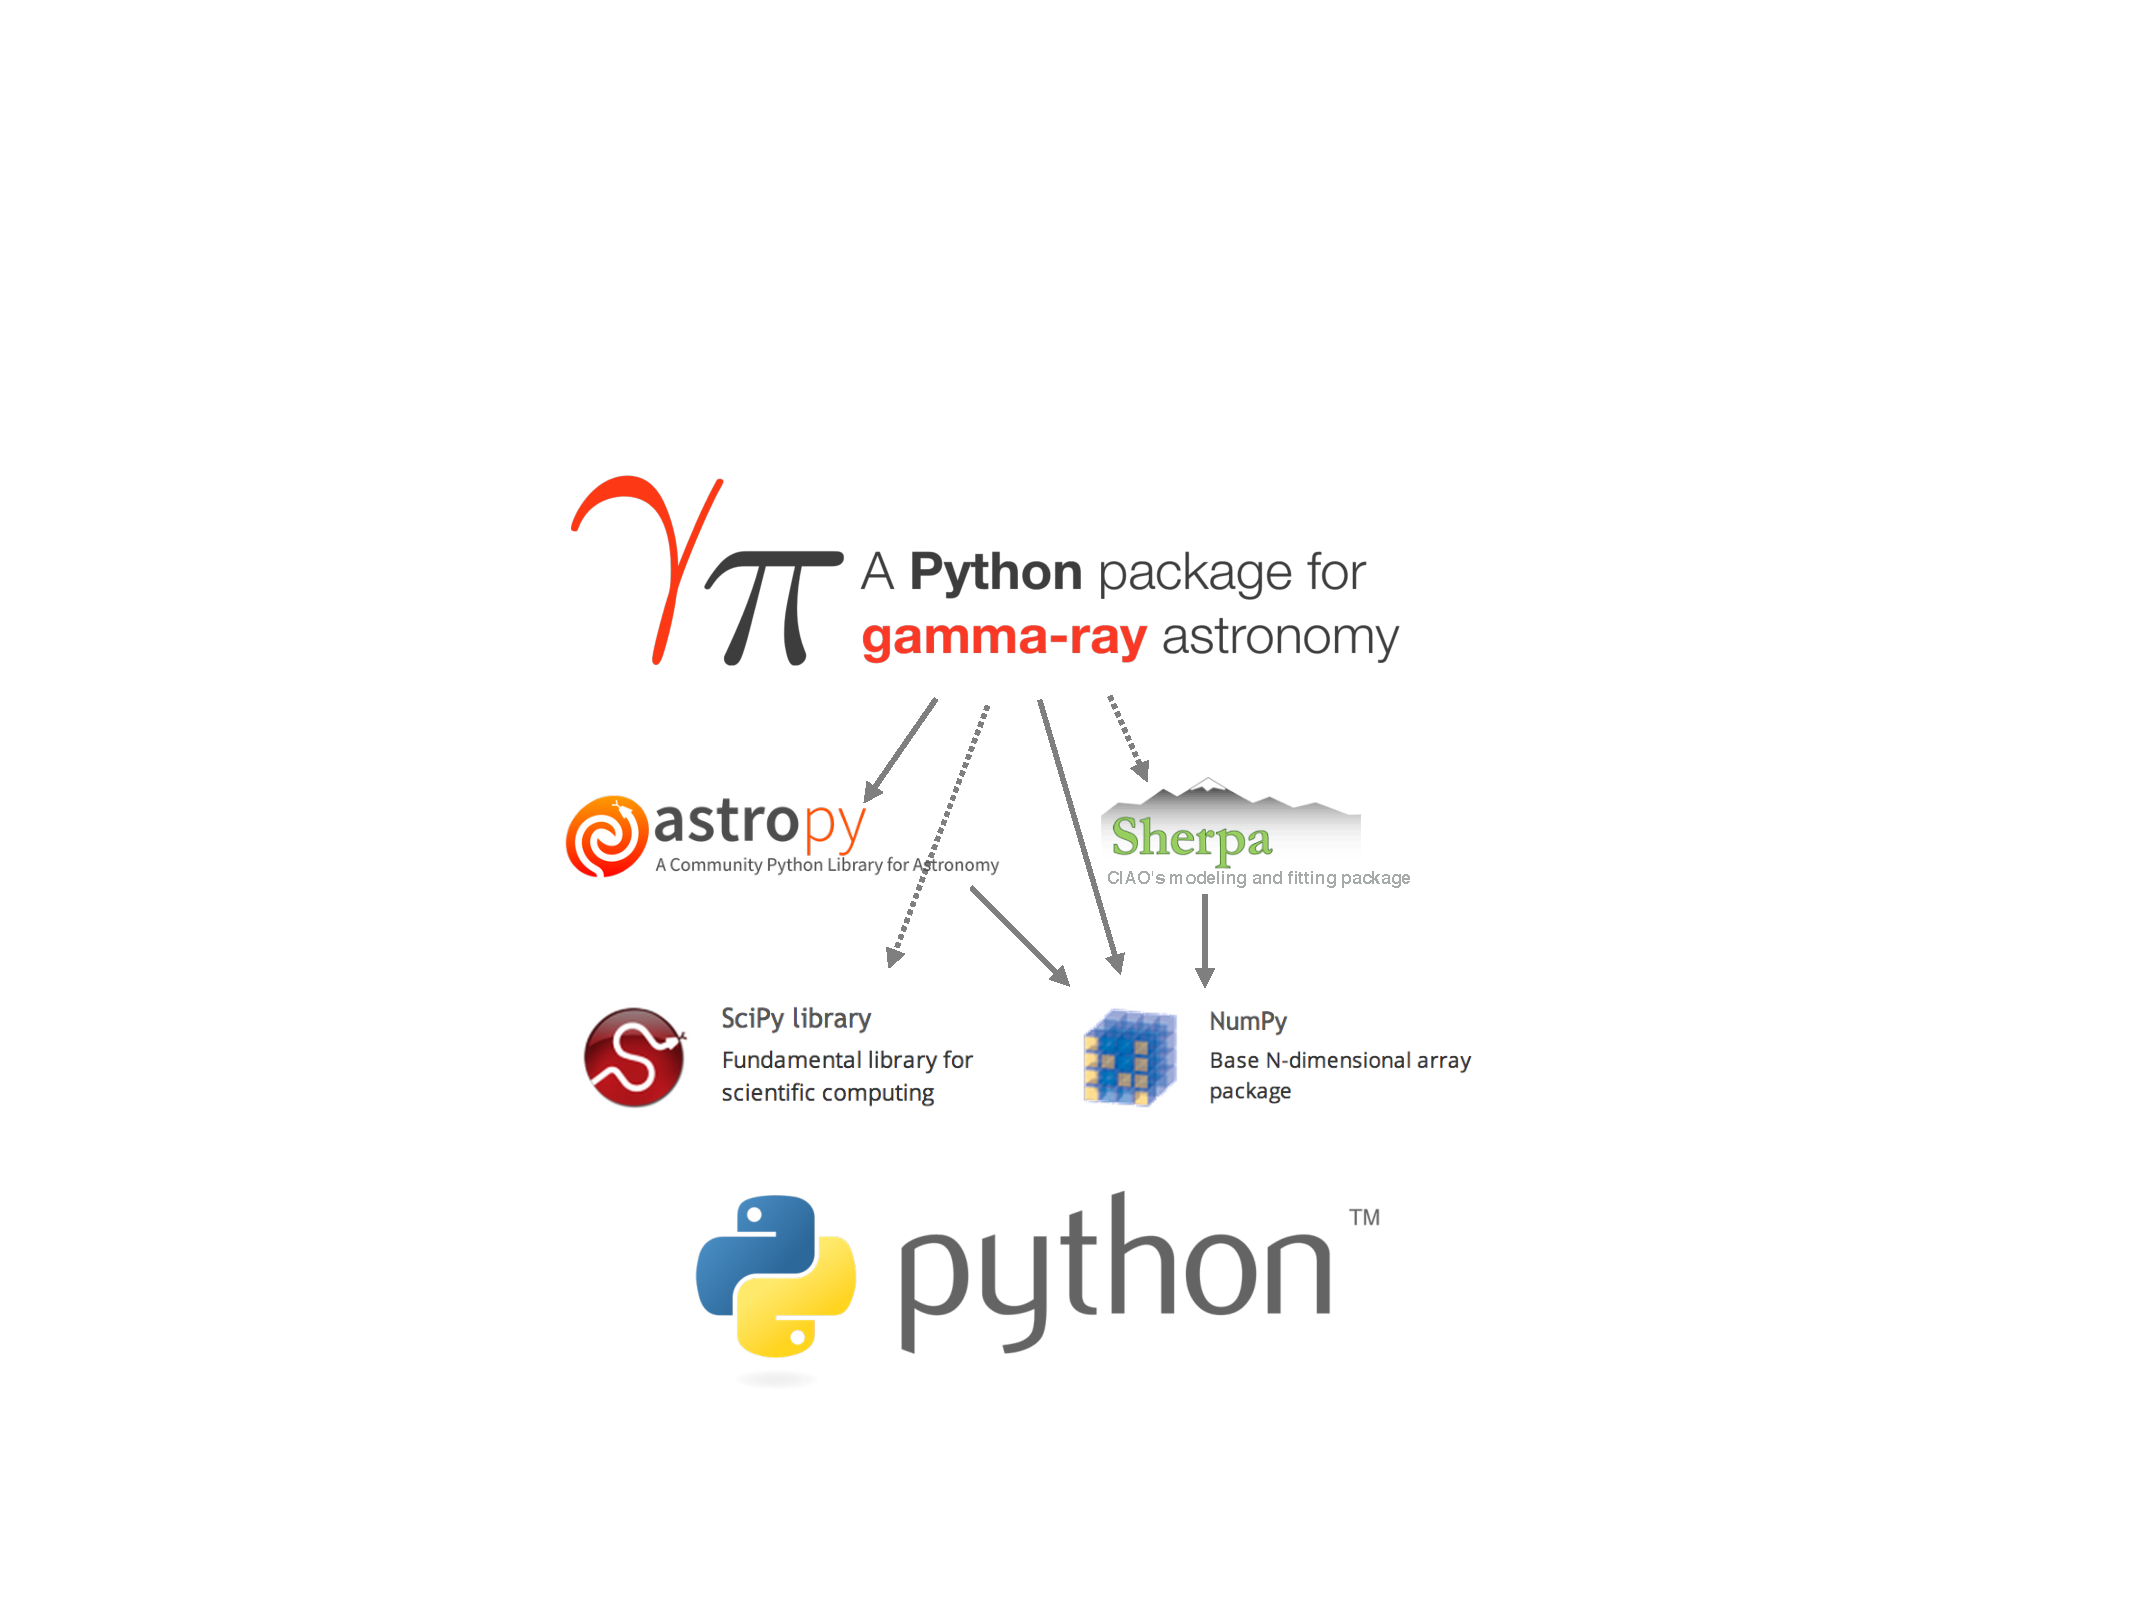
\includegraphics[width=0.7\textwidth]{figures/gammapy-stack}
\caption{
The Gammapy stack. Required dependencies Numpy and Astropy are illustrated with solid arrows, optional dependencies (the rest) with dashed arrows.
}
\label{fig:stack}
\end{figure}

\section{Code example}
\label{sec:code}

An example script using Gammapy is shown in Figure~\ref{fig:code_example}.

Message: Gammapy is high-level Python, data in Numpy arrays, others have written C and Python wrappers already (WCSLib, CFITSIO, SOFA/ERFA).

\begin{figure}[t]
\centering
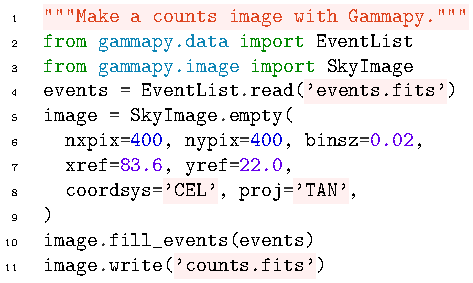
\includegraphics[width=0.5\textwidth]{examples/code_events_image}
\caption{
An example script using Gammapy to make a counts image from an event list.
This is used in Section~\ref{sec:code} to explain how Gammapy works.
TODO: probably should add a \texttt{def fill\_events(events, image)} function
and use that to illustrate how within Gammapy or in user scripts one can work
efficiently with events and pixels from Python, using Numpy arrays and
eventually calling into C extensions.
}
\label{fig:code_example}
\end{figure}


\section{Application example}
\label{sec:application}

TODO: add a CTA analysis example (probably only an image, no spectrum or
lightcurve yet). See
\url{https://nbviewer.jupyter.org/github/gammapy/gammapy-extra/blob/master/notebooks/cta\_data\_analysis.ipynb}
or if CTA-DC becomes available, a TS image from the Galactic plane survey would
be nice.

For further application examples see e.g. \cite{julien, roberta, cyril},
as well as \url{http://docs.gammapy.org}.

\section{Conclusions}
\label{sec:conclusions}

TODO: write me!

Briefly discuss Gammapy approach pro / con here or above?

\section{Acknowledgements}
\label{sed:acknowledgements}

This work was conducted in the context of the CTA Consortium.

We would like to thank the Scientific Python and specifically the Astropy
community for providing their packages which are invaluable to the development
of Gammapy, as well as tools and help with package setup and continuous
integration, as well as building of conda packages.

We thank the GitHub (\url{http://www.github.com}) team for providing us with an
excellent free development platform, ReadTheDocs (\url{https://readthedocs.org})
for free documentation hosting, Travis (\url{https://www.travis-ci.org}) and
Appveyor (\url{https://appveyor.com}) for free continuous integration testing,
and Slack (\url{https://slack.com/}) for a free team communication channel.


\bibliography{gammapy-icrc2017}
\bibliographystyle{JHEP}

\end{document}
